\documentclass[a4paper, UTF-8]{article}
\usepackage[margin=1in]{geometry}
\usepackage{algorithm}
\usepackage{algpseudocode}
\usepackage{amsmath}
\usepackage{pgfplots}
\usepackage{amsfonts}
\usepackage{amsthm}

\usepackage[utf8]{inputenc} % allow utf-8 input
\usepackage[T1]{fontenc}    % use 8-bit T1 fonts
\usepackage{hyperref}       % hyperlinks
\usepackage{url}            % simple URL typesetting
\usepackage{booktabs}       % professional-quality tables
\usepackage{amsfonts}       % blackboard math symbols
\usepackage{nicefrac}       % compact symbols for 1/2, etc.
\usepackage{microtype}      % microtypography
\usepackage{xcolor}         % colors

\theoremstyle{plain}
\newtheorem{theorem}{\indent Theorem}[section]
\newtheorem{lemma}[theorem]{\indent Lemma}
\newtheorem{assumption}{\indent Assumption}[section]
\newtheorem{note}[theorem]{\indent Notation}
\newtheorem{proposition}[theorem]{\indent Proposition}
\newtheorem{corollary}[theorem]{\indent Corollary}
\newtheorem{definition}{\indent Definition}[section]
\newtheorem{example}{\indent Example}[section]
\newtheorem{remark}{\indent Remark}[section]
\newenvironment{solution}{\begin{proof}[\indent\bf Solution]}{\end{proof}}
\renewcommand{\proofname}{\indent\bf Proof}

\begin{document}

\title{Assignment 4}

\author{Yanqiao Chen\\ 
  Department of Computer Science and Engineering\\
  Southern University of Science and Technology\\
  \texttt{12412115@mail.sustech.edu.cn}
  }


\maketitle

\section{Page 64, Problem 1}

% 1. 频率函数图 (Probability Mass Function)
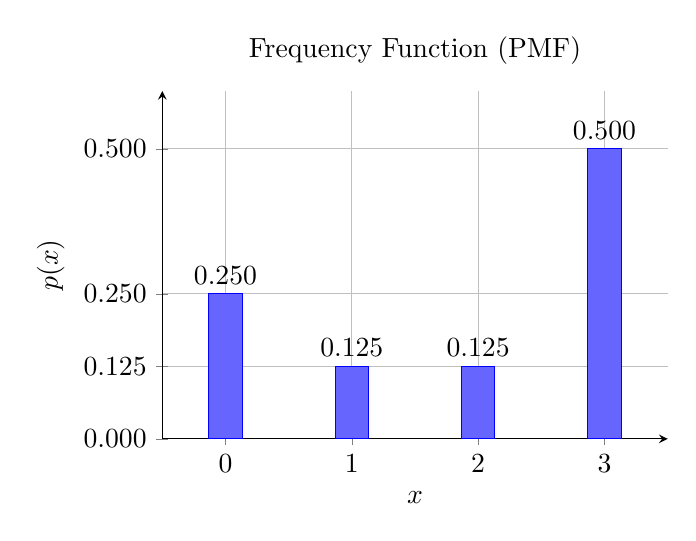
\begin{tikzpicture}
\begin{axis}[
    title={Frequency Function (PMF)},
    xlabel={$x$},
    ylabel={$p(x)$},
    ymin=0, ymax=0.6,
    xmin=-0.5, xmax=3.5,
    xtick={0,1,2,3},
    ytick={0.000,0.125,0.250,0.500},
  yticklabel style={
    /pgf/number format/fixed,
    /pgf/number format/precision=3,
    /pgf/number format/fixed zerofill
  },
    bar width=12pt,
    width=8cm,
    height=6cm,
    axis lines=left,
    grid=major
]
% 画柱状图
\addplot[ybar, fill=blue!60, draw=blue] coordinates {
  (0, 0.250)
    (1, 0.125)
    (2, 0.125)
  (3, 0.500)
};
% 标注数值
\node at (axis cs:0,0.250) [above] {0.250};
\node at (axis cs:1,0.125) [above] {0.125};
\node at (axis cs:2,0.125) [above] {0.125};
\node at (axis cs:3,0.500) [above] {0.500};
\end{axis}
\end{tikzpicture}

\vspace{1cm}

% 2. 累积分布函数图 (Cumulative Distribution Function)
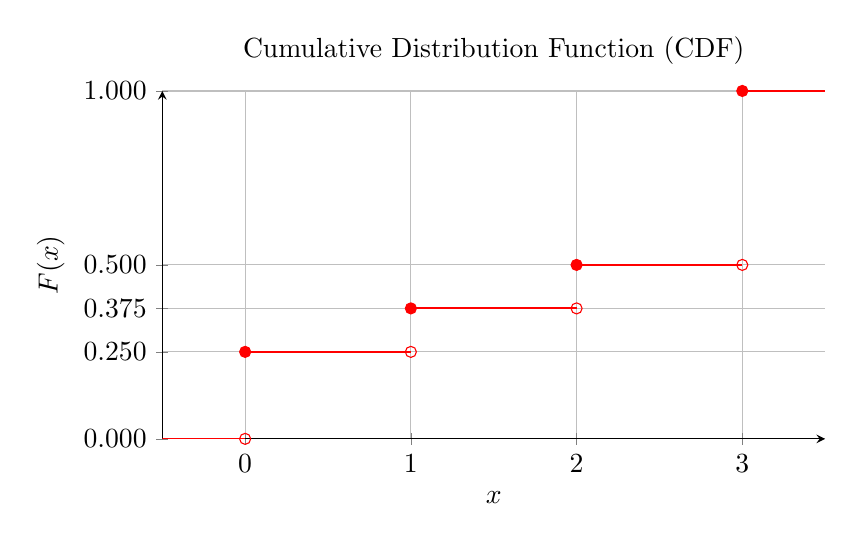
\begin{tikzpicture}
\begin{axis}[
  title={Cumulative Distribution Function (CDF)},
  xlabel={$x$},
  ylabel={$F(x)$},
  ymin= 0, ymax=1,
  xmin=-0.5, xmax=3.5,
  xtick={0,1,2,3},
  ytick={0.000,0.250,0.375,0.500,1.000},
  yticklabel style={
    /pgf/number format/fixed,
    /pgf/number format/precision=3,
    /pgf/number format/fixed zerofill
  },
  width=10cm,
  height=6cm,
  axis lines=left,
  grid=major
]
% 阶梯函数各水平线段
\addplot[red, thick] coordinates {(-0.5,0) (0,0)};
\addplot[red, thick] coordinates {(0,0.250) (1,0.250)};
\addplot[red, thick] coordinates {(1,0.375) (2,0.375)};
\addplot[red, thick] coordinates {(2,0.500) (3,0.500)};
\addplot[red, thick] coordinates {(3,1.000) (3.5,1.000)};

% 开圆点 (右端点不取)
\addplot[only marks, mark=o, mark options={draw=red, fill=white}, red]
coordinates {(0,0.000) (1,0.250) (2,0.375) (3,0.500)};

% 实心点 (右连续，在跳跃点处取上方值)
\addplot[only marks, mark=*, red]
coordinates {(0,0.250) (1,0.375) (2,0.500) (3,1.000)};
\end{axis}
\end{tikzpicture}


\section{Page 64, Problem 15}

Let the random variable $X$ be the number of team A wins. And $X \sim B(n, 0.4)$.  

In the three out of five games, the team A wins at least 3 games, so the probability is 

\begin{align*}
P(X \geq 3) &= P(X=3) + P(X=4) + P(X=5) \\
            &= \binom{5}{3} (0.4)^3 (0.6)^2 + \binom{5}{4} (0.4)^4 (0.6)^1 + \binom{5}{5} (0.4)^5 (0.6)^0 \\
            &= 0.31744 \\
\end{align*}

In the 4 out of 7 games, the team A wins at least 4 games, so the probability is
\begin{align*}
P(X \geq 4) &= P(X=4) + P(X=5) + P(X=6) + P(X=7) \\
            &= \binom{7}{4} (0.4)^4 (0.6)^3 + \binom{7}{5} (0.4)^5 (0.6)^2 + \binom{7}{6} (0.4)^6 (0.6)^1 + \binom{7}{7} (0.4)^7 (0.6)^0 \\
            &= 0.289792 \\
\end{align*}

Since $0.31744 > 0.289792$, it is to team A's advantage to play the best three out of five games.

\section{Page 64, Problem 31}

\subsection{a} 

From the formula we know
$$
P(X = k) = \frac{(\frac{1}{6} \times 2)^k}{k!}e^{-\frac{1}{6} \times 2} 
$$

Thus the probability that the phone rings at least once in the next 10 minutes is
\begin{align*}
P(X \geq 1) &= 1 - P(X=0) \\
            &= 1 - e^{-\frac{1}{6} \times 2} \\
            &\approx 0.2835
\end{align*}

\subsection{b} 

Let the time length be $T$, we have 
$$
P(X = 0) = e^{-2 \times T} \leq 0.5
$$

Thus, we obtain 
$$
2T \geq \ln 2 \Rightarrow T \geq \frac{\ln 2}{2} \approx 0.3466
$$

Thus the answer is at least approximately 0.3466 hours, which is about 20.8 minutes.

\section{Supplementary Problem 1.1}

\begin{align*} 
    P(X = 1) = c\times \frac{2}{3} \\ 
    P(X = 2) = c\times \frac{4}{9} \\
    P(X = 3) = c\times \frac{8}{27} \\
\end{align*}

And 
$$
c(\frac{2}{3} + \frac{4}{9} + \frac{8}{27}) =  c \cdot \frac{38}{27} = 1
$$

Thus we can obtain $c = \frac{27}{38}$.

\section{Supplementary Problem 1.2}

$$
P(X = k) = \frac{\lambda^k}{k!}e^{-\lambda}
$$

Let 
$$
P(X = k) \geq P(X = k-1) \Rightarrow \frac{\lambda^k}{k!}e^{-\lambda} \geq \frac{\lambda^{k-1}}{(k-1)!}e^{-\lambda} \Rightarrow \lambda \geq k
$$

and 
$$
P(X = k) \geq P(X = k+1) \Rightarrow \frac{\lambda^k}{k!}e^{-\lambda} \geq \frac{\lambda^{k+1}}{(k+1)!}e^{-\lambda} \Rightarrow \lambda - 1\leq k
$$

Thus we can obtain
$$
\lambda - 1 \leq k \leq \lambda
$$

Thus we obtain the probability that $X$ takes the value of $k$ is the largest is
\begin{align*} 
    k = \begin{cases}
    \lambda - 1 \text{ or } \lambda, & \text{if } \lambda \text{ is an integer} \\
    \lfloor\lambda\rfloor, & \text{otherwise}
    \end{cases}
\end{align*}


\section{Supplementary Problem 1.3}

\subsection{a} 

The frequency function of $X$ is

$$
P(X = x) = \frac{\binom{2}{x}\binom{13}{3-x}}{\binom{15}{3}}, x = 0, 1, 2
$$

\subsection{b} 

The distribution function of $X$ is
\begin{align*}
P(X \leq x) = \begin{cases}
0, & x < 0 \\
\frac{22}{35}, & 0 \leq x < 1 \\
\frac{34}{35}, & 1 \leq x < 2 \\
1, & 2 \leq x 
\end{cases}
\end{align*}

\subsection{c} 

$$
P(X \leq \frac{1}{2}) = \frac{22}{35}
$$

$$
P(1 < X \leq \frac{3}{2}) = P(X \leq \frac{3}{2}) - P(X \leq 1) = 0
$$

$$
P(1 \leq X \leq \frac{3}{2}) = P(X \leq \frac{3}{2}) - P(X \leq 1) + P(X = 1) = \frac{12}{35}
$$

$$
P(1 < X < 2) = P(X \leq 2) - P(X \leq 1) - P(X = 2) = 0
$$

\section{Supplementary Problem 1.4} 

\subsection{a}

Let $X$ represents the number of the people that dies in the year. We have $X \sim B(2500, 0.002)$. The total profit is $30000 - 2000X$.

Thus the probability that the company have a deficit is 
$$
P(30000 - 2000X < 0) = P(X > 15) = 1 - P(X \leq 15) = 1 - \sum_{k=0}^{15} \binom{2500}{k} (0.002)^k (0.998)^{2500-k}
$$

\subsection{b}

The probability that the company have a profit over 10000 is 
$$
P(30000 - 2000X > 10000) = P(X < 10) = \sum_{k=0}^{9} \binom{2500}{k} (0.002)^k (0.998)^{2500-k}
$$

The probability that the company have a profit over 20000 is 
$$
P(30000 - 2000X > 20000) = P(X < 5) = \sum_{k=0}^{4} \binom{2500}{k} (0.002)^k (0.998)^{2500-k}
$$
We omit the accurate numerical calculation here.

\begin{remark}
Since $n$ is relatively large and $p$ is relatively small, we can use the Poisson distribution to approximate the Binomial distribution. Let $\lambda = np = 2500 \times 0.002 = 5$. Thus we have $X \sim P(5)$.

Thus the probability that the company have a deficit is
$$
P(X > 15) = 1 - P(X \leq 15) \approx 1 - \sum_{k=0}^{15} \frac{5^k}{k!}e^{-5} \approx 6.90 \times 10^{-5}
$$

The probability that the company have a profit over 10000 is
$$
P(X < 10) \approx \sum_{k=0}^{9} \frac{5^k}{k!}e^{-5} \approx 0.9682
$$

The probability that the company have a profit over 20000 is
$$
P(X < 5) \approx \sum_{k=0}^{4} \frac{5^k}{k!}e^{-5} \approx 0.4405
$$

\end{remark}

\end{document}